% mnras_template.tex 
%
% LaTeX template for creating an MNRAS paper
%
% v3.0 released 14 May 2015
% (version numbers match those of mnras.cls)
%
% Copyright (C) Royal Astronomical Society 2015
% Authors:
% Keith T. Smith (Royal Astronomical Society)

% Change log
%
% v3.0 May 2015
%    Renamed to match the new package name
%    Version number matches mnras.cls
%    A few minor tweaks to wording
% v1.0 September 2013
%    Beta testing only - never publicly released
%    First version: a simple (ish) template for creating an MNRAS paper

%%%%%%%%%%%%%%%%%%%%%%%%%%%%%%%%%%%%%%%%%%%%%%%%%%
% Basic setup. Most papers should leave these options alone.
\documentclass[fleqn,usenatbib]{mnras}

% MNRAS is set in Times font. If you don't have this installed (most LaTeX
% installations will be fine) or prefer the old Computer Modern fonts, comment
% out the following line
\usepackage{newtxtext,newtxmath}
% Depending on your LaTeX fonts installation, you might get better results with one of these:
%\usepackage{mathptmx}
%\usepackage{txfonts}

% Use vector fonts, so it zooms properly in on-screen viewing software
% Don't change these lines unless you know what you are doing
\usepackage[T1]{fontenc}

% Allow "Thomas van Noord" and "Simon de Laguarde" and alike to be sorted by "N" and "L" etc. in the bibliography.
% Write the name in the bibliography as "\VAN{Noord}{Van}{van} Noord, Thomas"
\DeclareRobustCommand{\VAN}[3]{#2}
\let\VANthebibliography\thebibliography
\def\thebibliography{\DeclareRobustCommand{\VAN}[3]{##3}\VANthebibliography}


%%%%% AUTHORS - PLACE YOUR OWN PACKAGES HERE %%%%%

% Only include extra packages if you really need them. Common packages are:
\usepackage{graphicx}	% Including figure files
\usepackage{amsmath}	% Advanced maths commands
% \usepackage{amssymb}	% Extra maths symbols

\usepackage{caption}
\usepackage{subcaption}
\graphicspath{{figures/}}
% \usepackage{verbatim}
\usepackage{booktabs}
\usepackage{threeparttable}
\usepackage{makecell}

\usepackage{siunitx}
\sisetup{
	separate-uncertainty = true,
    tight-spacing = false,
    % table-alignment-mode = marker,
    % table-number-alignment = center
	% inter-unit-product = \ensuremath{{}\cdot{}}
}
\DeclareSIUnit\angstrom{\text{\AA}}

\usepackage[version=4]{mhchem}
\usepackage[calc]{datetime2}
% \usepackage{datetime2-calc}
\DTMnewdatestyle{mnras}{  % set the date format for mnras
    \renewcommand{\DTMdisplaydate}[4]{##1 \pgfcalendarmonthname{##2} \number##3 }
    \renewcommand{\DTMDisplaydate}{\DTMdisplaydate}
}
\DTMsetdatestyle{mnras}
% \DTMtryregional{en}{GB}
% \DTMsetdatestyle{default} % default iso yyyymd ddmmyyyy
% \DTMsetup{datesep={/}}
% \usepackage{soul}
% \setulcolor{blue}
% \setstcolor{red}
% \sethlcolor{yellow}
% \soulregister\cite7
% \soulregister\ref7
% \soulregister\autoref7
% \soulregister\citep7
% \soulregister\citet7
% \soulregister\citealp7
% \soulregister\citealt7
% \soulregister\pageref7
% \soulregister{\textbf}{7}
% \soulregister{\href}{1}
% \soulregister{\si}{7}
% \soulregister{\qty}{1}
% \soulregister{\SI}{1}
% \soulregister{\ang}{7}
% \soulregister{\num}{7}
% \soulregister{\ce}{7}
% \soulregister\DTMdate7
% \soulregister\texttt7

\usepackage[defaultcolor=orange]{changes}

\newcommand*{\dif}{\mathop{}\!\mathrm{d}}

% \usepackage{showframe} 	% some manual settings

%%%%%%%%%%%%%%%%%%%%%%%%%%%%%%%%%%%%%%%%%%%%%%%%%%

%%%%% AUTHORS - PLACE YOUR OWN COMMANDS HERE %%%%%

% Please keep new commands to a minimum, and use \newcommand not \def to avoid
% overwriting existing commands. Example:
%\newcommand{\pcm}{\,cm$^{-2}$}	% per cm-squared

%%%%%%%%%%%%%%%%%%%%%%%%%%%%%%%%%%%%%%%%%%%%%%%%%%

%%%%%%%%%%%%%%%%%%% TITLE PAGE %%%%%%%%%%%%%%%%%%%

% Title of the paper, and the short title which is used in the headers.
% Keep the title short and informative.
\title[Short title, max. 45 characters]{Broadband CCD photometry of Long-period comets C/2019 L3 (ATLAS) and C/2020 P3 (ATLAS)}

% The list of authors, and the short list which is used in the headers.
% If you need two or more lines of authors, add an extra line using \newauthor
\author[K. T. Smith et al.]{
Keith T. Smith,$^{1}$\thanks{E-mail: publications@ras.ac.uk (KTS)}
A. N. Other,$^{2}$
Third Author$^{2,3}$
and Fourth Author$^{3}$
\\
% List of institutions
$^{1}$Royal Astronomical Society, Burlington House, Piccadilly, London W1J 0BQ, UK\\
$^{2}$Department, Institution, Street Address, City Postal Code, Country\\
$^{3}$Another Department, Different Institution, Street Address, City Postal Code, Country
}

% These dates will be filled out by the publisher
\date{Accepted XXX. Received YYY; in original form ZZZ}

% Enter the current year, for the copyright statements etc.
\pubyear{\DTMfetchyear{now}}

% Don't change these lines
\begin{document}
\label{firstpage}
\pagerange{\pageref{firstpage}--\pageref{lastpage}}
\maketitle

\DTMsavenow{now}

% Abstract of the paper
\begin{abstract}
This is a simple template for authors to write new MNRAS papers.
The abstract should briefly describe the aims, methods, and main results of the paper.
It should be a single paragraph not more than 250 words (200 words for Letters).
No references should appear in the abstract.
\end{abstract}

% Select between one and six entries from the list of approved keywords.
% Don't make up new ones.
\begin{keywords}
keyword1 -- keyword2 -- keyword3
\end{keywords}

%%%%%%%%%%%%%%%%%%%%%%%%%%%%%%%%%%%%%%%%%%%%%%%%%%

%%%%%%%%%%%%%%%%% BODY OF PAPER %%%%%%%%%%%%%%%%%%

\section{Introduction}

As primitive objects in the Solar System, comets have the same physical and chemical properties as the planetary systems in the early Solar System, which can reveal information about the early Solar System \citep{solontoi_ensemble_2012}. Research on comets can let us further understand the mechanism of planet formation and even solve some basic questions such as the origin of water on Earth \citep{alexander_water_2018}. Unlike Short-peroid comets ($\mathrm{P}<\qty{200}{yr}$), most Long-period comets ($\mathrm{P}>\qty{200}{yr}$) originate from the Oort Cloud and are entering the inner Solar System for the first time. Long-period comets tend to exhibit stronger activity characteristics than Short-peroid comets do and appear brighter visually at the same heliocentric distance due to the more volatile components they contain, comparing with the conventional water ice. 

Long-period comets also exhibit activity at large heliocentric distances more than {\qty{5}{\astronomicalunit}}. At this time, the activity is not caused by the sublimation effect of water ice. The current explanation about distant activity of comets mainly includes: the phase transition between amorphous and crystalline water ice~\citep{prialnik_crystallization_1992, capria_c1995_2002}, the annealing of amorphous water ice \citep{meech_activity_2009}, and the sublimation of more volatile components such as \ce{CO2}~\citep{ootsubo_akari_2012} and/or \ce{CO}~\citep{jewitt_distant_2019}. 
% For comets that are active at a heliocentric distance of more than {\SI{4}{\astronomicalunit}} and whose nucleus surface temperature is lower than the \ce{H2O} sublimation temperature, their activity may be caused by the sublimation of more volatile \ce{CO2}~\citep{ootsubo_akari_2012} or \ce{CO}~\citep{jewitt_distant_2019}. In addition, \citet{ivanova_observations_2011} show that the upper layer of the comet nucleus should continue to peel off in order to conform to the observation results of long-term high activity of comets. 

Two Long-period comets C/2019 L3 and C/2020 P3 are selected for this study. They are all nearly isotropic, both of them having orbital semi-major axis more than {\qty{10000}{\astronomicalunit}}. C/2019 L3 and C/2020 P3 reach their perihelion on \DTMdate{2022-1-9} and \DTMdate{2021-4-21}, respectively. Fig.~\ref{fig:orbit} shows the planar orbit graph of two comets in the Solar System. Table~\ref{tab:orb_elem} is the summary on orbital elements of these two comets. 

In this paper, we present broadband CCD photometry results of comets C/2019 L3 and C/2020 P3. The circumstance of observations and data reduction process are presented in Section \ref{sec:obs_data}. Section \ref{sec:res} describes the photometry results, including morphology, surface brightness, $Af\rho$ and coma colors. Finally, discussion and conclusions are presented in Section \ref{sec:dis} and Section \ref {sec:con}. 

% orbital graph
\begin{figure}
    \centering
    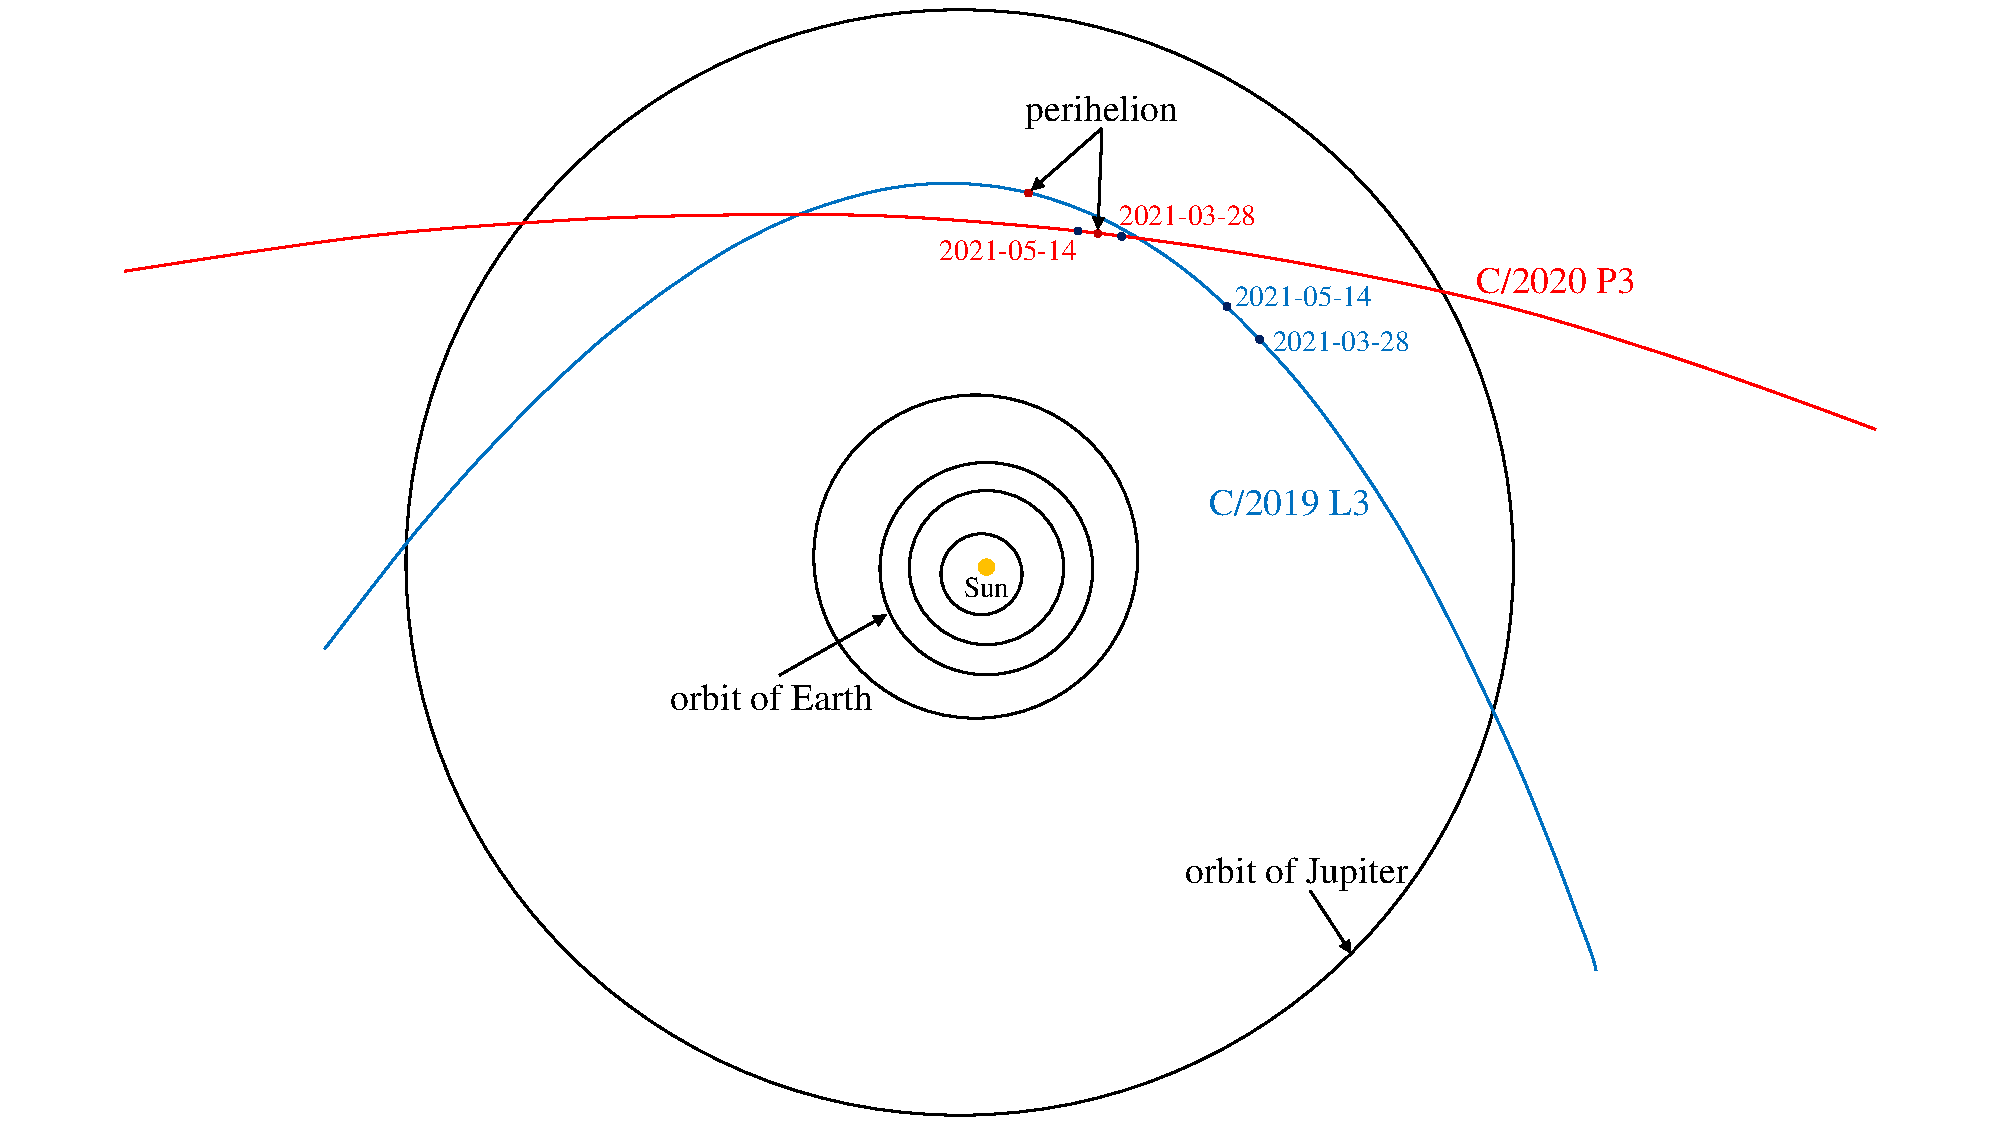
\includegraphics[width=1.0\columnwidth]{orbit.pdf}
    \caption{Orbit of comets C/2019 L3 and C/2020 P3 in the Solar System. The blue curve is the orbit of C/2019 L3 and the red curve is the orbit of C/2020 P3. Closed curves in black are the orbits of planets in the Solar System. Note that both of these comets have large orbital inclination not shown in this planar graph. The start and end dates of observations as well as the corresponding position of two objects on these dates are marked in this graph. }
    \label{fig:orbit}
\end{figure}

% orbital elements
\begin{table}
    \centering
    \caption{Orbital elements of comets C/2019 L3 and C/2020 P3 (Epoch: \DTMdate{2022-7-19}). }\label{tab:orb_elem}
    \begin{threeparttable}
        \resizebox{\linewidth}{!}{
        \begin{tabular}{ccccccccc}
            \toprule
            Comet & e\tnote{1} & q\tnote{2} & i\tnote{3} & $\Omega$\tnote{4} & $\omega$\tnote{5} & L\tnote{6} & B\tnote{7} & T\tnote{8} \\
            \midrule
            C/2019 L3       & \num{1.0017730}  & \num{3.5544290}  & \num{48.35710}  & \num{290.78850}  & \num{171.60970}  & \num{285.19094}  & \num{6.26014}   & \num{2459589.11650}  \\
            C/2020 P3       & \num{1.0003270}  & \num{6.8123330}  & \num{61.88790}  & \num{19.46850}   & \num{82.25590}   & \num{93.37021}   & \num{60.92485}  & \num{2459325.45200} \\
            \bottomrule
        \end{tabular}
        }
% 在正文介绍classification的部分
        \begin{tablenotes}
            \item[1] eccentricity 
            \item[2] perihelion distance
            \item[3] inclination
            \item[4] Longitude of ascending node
            \item[5] Argument of perihelion
            \item[6] Longitude of perihelion
            \item[7] Latitude of perihelion
            \item[8] Time of perihelion passage
        \end{tablenotes}
    \end{threeparttable}
\end{table}


\section{Methods, Observations, Simulations etc.}

Normally the next section describes the techniques the authors used.
It is frequently split into subsections, such as Section~\ref{sec:maths} below.

\subsection{Maths}
\label{sec:maths} % used for referring to this section from elsewhere

Simple mathematics can be inserted into the flow of the text e.g. $2\times3=6$
or $v=220$\,km\,s$^{-1}$, but more complicated expressions should be entered
as a numbered equation: 

\begin{equation}
    x=\frac{-b\pm\sqrt{b^2-4ac}}{2a}.
	\label{eq:quadratic}
\end{equation}

Refer back to them as e.g. equation~(\ref{eq:quadratic}).

\subsection{Figures and tables}

Figures and tables should be placed at logical positions in the text. Don't
worry about the exact layout, which will be handled by the publishers.

Figures are referred to as e.g. Fig.~\ref{fig:example_figure}, and tables as
e.g. Table~\ref{tab:example_table}.

% Example figure
\begin{figure}
	% To include a figure from a file named example.*
	% Allowable file formats are eps or ps if compiling using latex
	% or pdf, png, jpg if compiling using pdflatex
	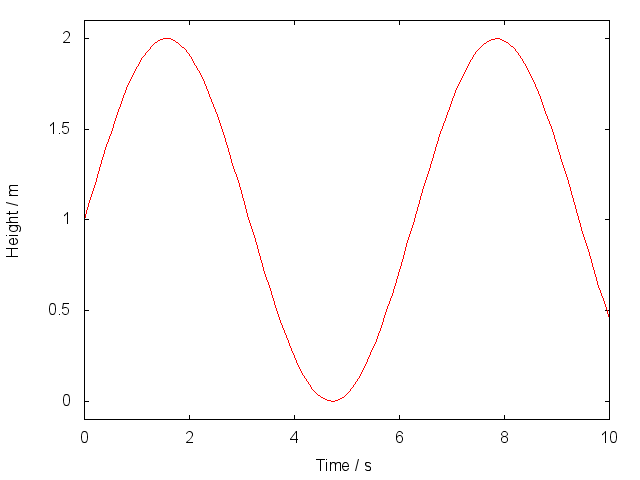
\includegraphics[width=\columnwidth]{example}
    \caption{This is an example figure. Captions appear below each figure.
	Give enough detail for the reader to understand what they're looking at,
	but leave detailed discussion to the main body of the text.}
    \label{fig:example_figure}
\end{figure}

% Example table
\begin{table}
	\centering
	\caption{This is an example table. Captions appear above each table.
	Remember to define the quantities, symbols and units used.}
	\label{tab:example_table}
	\begin{tabular}{lccr} % four columns, alignment for each
		\hline
		A & B & C & D\\
		\hline
		1 & 2 & 3 & 4\\
		2 & 4 & 6 & 8\\
		3 & 5 & 7 & 9\\
		\hline
	\end{tabular}
\end{table}


\section{Conclusions}

The last numbered section should briefly summarise what has been done, and describe
the final conclusions which the authors draw from their work.

\section*{Acknowledgements}

The Acknowledgements section is not numbered. Here you can thank helpful
colleagues, acknowledge funding agencies, telescopes and facilities used etc.
Try to keep it short.

%%%%%%%%%%%%%%%%%%%%%%%%%%%%%%%%%%%%%%%%%%%%%%%%%%
\section*{Data Availability}

 
The inclusion of a Data Availability Statement is a requirement for articles published in MNRAS. Data Availability Statements provide a standardised format for readers to understand the availability of data underlying the research results described in the article. The statement may refer to original data generated in the course of the study or to third-party data analysed in the article. The statement should describe and provide means of access, where possible, by linking to the data or providing the required accession numbers for the relevant databases or DOIs.




%%%%%%%%%%%%%%%%%%%% REFERENCES %%%%%%%%%%%%%%%%%%

% The best way to enter references is to use BibTeX:

\bibliographystyle{mnras}
\bibliography{example} % if your bibtex file is called example.bib


% Alternatively you could enter them by hand, like this:
% This method is tedious and prone to error if you have lots of references
%\begin{thebibliography}{99}
%\bibitem[\protect\citeauthoryear{Author}{2012}]{Author2012}
%Author A.~N., 2013, Journal of Improbable Astronomy, 1, 1
%\bibitem[\protect\citeauthoryear{Others}{2013}]{Others2013}
%Others S., 2012, Journal of Interesting Stuff, 17, 198
%\end{thebibliography}

%%%%%%%%%%%%%%%%%%%%%%%%%%%%%%%%%%%%%%%%%%%%%%%%%%

%%%%%%%%%%%%%%%%% APPENDICES %%%%%%%%%%%%%%%%%%%%%

\appendix

\section{Some extra material}

If you want to present additional material which would interrupt the flow of the main paper,
it can be placed in an Appendix which appears after the list of references.

%%%%%%%%%%%%%%%%%%%%%%%%%%%%%%%%%%%%%%%%%%%%%%%%%%


% Don't change these lines
\bsp	% typesetting comment
\label{lastpage}
\end{document}

% End of mnras_template.tex
